\documentclass{classrep}
\usepackage[utf8]{inputenc}
\usepackage{amsmath}
\usepackage{graphicx}
\usepackage{url}
\usepackage{hyperref}
\usepackage[T1]{fontenc}
\usepackage[polish]{babel}
\usepackage[utf8]{inputenc}
\usepackage{lmodern}
\usepackage{color}
\selectlanguage{polish}
\graphicspath{ {./rys/} }



\studycycle{Informatyka, studia dzienne, inż I st.}
\coursesemester{VI}

\coursename{Sztuczna inteligencja i systemy ekspertowe}
\courseyear{2019/2020}

\courseteacher{dr inż. Krzysztof Lichy}
\coursegroup{wtorek, 10:30}

\author{
  \studentinfo{Radosław Grela}{216769} \and
  \studentinfo{Jakub Wąchała}{216914}
}

\title{Zadanie 1: Piętnastka}

\begin{document}
\maketitle

\newpage

\section{Cel}
W tym zadaniu należało napisać program, który będzie rozwiązywał układankę pod nazwą \textsl{Piętnastka (Fifteen Puzzle)}.
Następnie, należało przebadać układy początkowe układanki w odległościach 1-7 od układu wzorcowego (413 układów)
korzystając z różnych strategii i przypadków przeszukiwania sąsiedztwa.

\section{Wprowadzenie}
\textsl{Piętnastka}, potocznie też \textsl{Przesuwanka} to prosta gra logiczna, w której zadaniem jest ułożyć 15 ponumerowanych kwadratowych klocków umieszczonych w pudełku 4x4. Pozostałe, 16 miejsce jest puste, co pozwala na poruszanie elementów układanki.\cite{pierwszymath} 
\begin{figure}[h!]
    \centering
    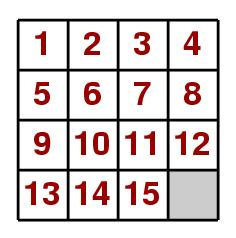
\includegraphics[width=0.25\textwidth]{15grid1.jpg}
    \caption{Ułożona piętnastka. \cite{pierwszymath}}
\end{figure}

W programie przez nas napisanym mamy do wyboru 3 strategie przestrzeni stanów:
\begin{itemize}
\item Strategia wszerz BFS (\textsl{breadth-first search})
\item Strategia w głąb DFS(\textsl{depth-first search})
\item Strategia najpierw najlepszy A* z heurystykami Hamminga i Manhattan
\end{itemize}
Strategie te są przykładem przeszukiwania drzewa. Jego węzłami są stany, czyli aktualne ułożenia układanki.
W części badawczej badaliśmy tylko układanki rozmiarów 4x4, jednak nasz program dopuszcza także niestandardowe rozmiary.

\subsection{DFS}
Badanie grafu strategią DFS polega na przejściu wszystkich krawędzi wychodzących z podanego wierzchołka. Jest to algorytm rekurencyjny. Kolejność przechodzenia po drzewie przedstawiona jest na poniższym rysunku:
 \begin{figure}[h!]
    \centering
    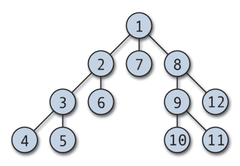
\includegraphics[width=0.5\textwidth]{dfs.png}
    \caption{Kolejność przechodzenia w algorytmie DFS. \cite{wikiDFS}}
\end{figure}

Gdy rozwiązanie zostanie znalezione, wystarczy wrócić rekurencyjnie do rodzica.

\subsection{BFS}
Algorytm BFS polega na przejściu przez wszystkich sąsiadów danego wierzchołka. Następnie, należy kontynuować czynność dalej, dopóki nie odwiedzimy wszystkich sąsiadów sąsiadów. Kolejność przechodzenia po drzewie jest następująca:
\begin{figure}[h!]
    \centering
    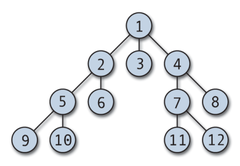
\includegraphics[width=0.5\textwidth]{bfs.png}
    \caption{Kolejność przechodzenia w algorytmie BFS. \cite{wikiBFS}}
\end{figure}

\subsection{A*}
A* to kolejna strategia przeszukiwania grafu. Bazuje ona na funkcji 
\begin{equation}
f(x) = g(x) + h(x) 
\label{fun}
\end{equation}
gdzie $g(x)$ oznacza głębokość, a $h(x)$ to wartość odpowiedniej funkcji miary błędu. W naszym programie wykorzystujemy następujące dwie metryki:
\subsubsection{Metryka Hamminga}
W metryce Hamminga jako wynik funkcji $h(x)$ podawana jest ilość klocków, która nie znajduje się na swojej pozycji. Przykładowo dla układanki na rysunku (\ref{blednaukladanka}) wynik takiej funkcji będzie równy 4 (elementy 3, 4, 8 i 12 nie znajdują się na swoich pozycjach).
\begin{figure}[h!]
    \centering
    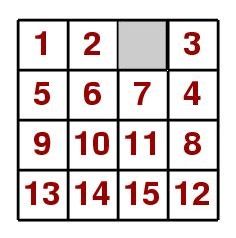
\includegraphics[width=0.25\textwidth]{15wrong1.jpg}
    \caption{Przykładowa błędnie ułożona układanka.}
	\label{blednaukladanka}
\end{figure}

\subsubsection{Metryka Manhattan}
W tej metryce wynikiem funkcji $h(x)$ jest suma wartości bezwzględnych różnic współrzędnych między punktem, w którym klocek powinien się znaleźć, a punktem, w którym jest obecnie. Dla rysunku (\ref{blednaukladanka}) wynik to 8 (4 + 1 + 1 + 1 + 1).

\section{Opis implementacji}
Napisany przez nas program jest aplikacją konsolową napisaną w języku Java. Jako parametry programu należy podać 5 argumentów:
\begin{enumerate}
\item strategia (dfs, bfs, astr)
\item porządek (jeżeli jest to strategia DFS lub BFS) lub heurystyka (dla metody A*). 
\item ścieżka do pliku z zadaną układanką do ułożenia
\item ścieżka do pliku, w którym zostanie zapisane rozwiązanie
\item ścieżka do pliku, w którym zostaną zapisane dodatkowe informacje dot. przeprowadzonego procesu
\end{enumerate}
Poniżej przedstawiamy krótki opis, jak zostały zaimplementowane poszczególne strategie.
\subsection{DFS}
Do przechowywania stanów nie używamy specjalnej struktury danych, lecz za pomocą rekurencji program wie, który węzęł musi odwiedzić jako następny. Zatem przechowywanie stanów jest możliwe dzięki odkładaniu wywołań funkcji na stosie.
\subsection{BFS}
{\color{red} elo here do napisania}

\subsection{A*}
W przypadku algorytmów A* dane są przetrzymywane na liście (ArrayList), która spełnia zadania kolejki priorytetowej. W momencie dodania nowego elementu na liście, jest ona sortowana zgodnie z wynikiem funkcji (\ref{fun}). Na początku listy znajdują się ''najgorsze'' elementy - te, których wartość funkcji jest największa, a na końcu elementy, które mają wartość tej funkcji najmniejszą.

Na poniższym rysunku przedstawiony jest diagram UML naszego programu.
\begin{figure}[h!]
    \centering
    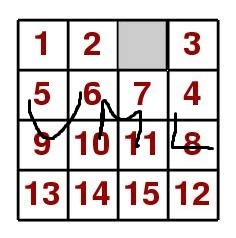
\includegraphics[width=0.4\textwidth]{uml.jpg}
    \caption{Diagram UML.}
\end{figure}
\newpage

\section{Materiały i metody}
Do przeprowadzenia badań nad utworzoną przez nas aplikacją użyliśmy kilku programów znajdujących się na stronie przedmiotu na Wikampie.
\begin{enumerate}
\item Program do utworzenia 413 różnych układów piętnastki z głębokością 1-7
\item Skrypt uruchamiający naszą aplikację z każdym algorytmem oraz ewentualną heurystyką i kolejnością
\item Skrypt Podsumowujący uzyskane wyniki z poprzedniego skryptu
\end{enumerate}
Otrzymane wyniki przedstawiliśmy na wykresach w następnej sekcji.

\section{Wyniki}
Na poniższych wykresach przedstawiliśmy średnie wartości:
\begin{itemize}
\item Czasu wykonywania
\item Maksymalnej głębokości
\item Ilości przetworzonych węzłów
\item Ilości odwiedzonych węzłów
\item Długości rozwiązania
\end{itemize}
Każdy wykres został wykonany dla każdej strategii oraz ich heurystyk.

\begin{figure}[h!]
    \centering
    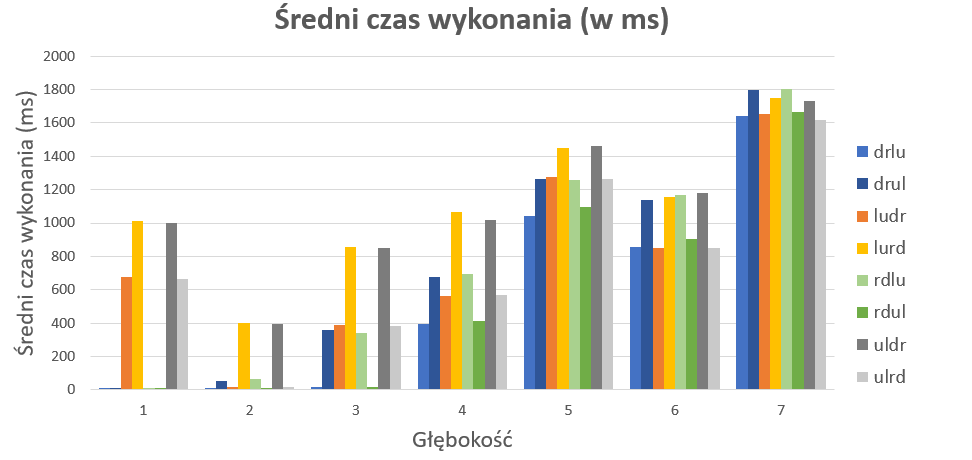
\includegraphics[width=0.85\textwidth]{czasdfs.png}
    \caption{Średni czas wykonania dla algorytmu DFS}
	\label{czasdfs}
\end{figure}
\begin{figure}[h!]
    \centering
    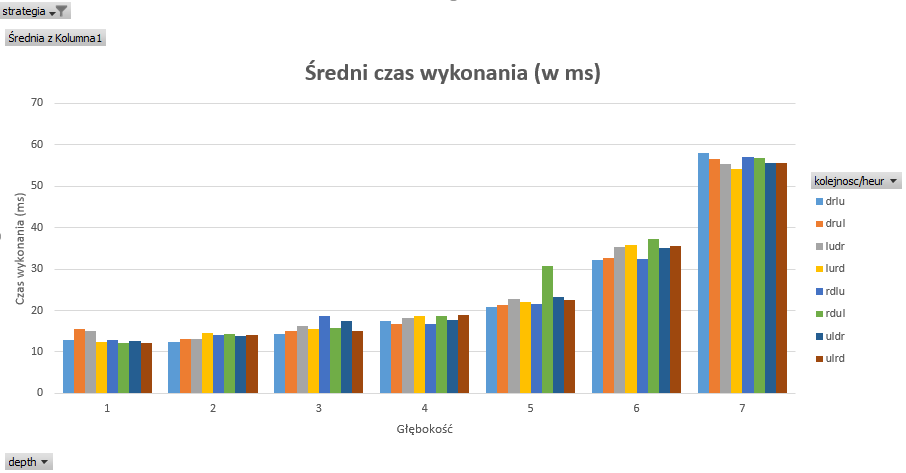
\includegraphics[width=0.85\textwidth]{czasbfs.png}
    \caption{Średni czas wykonania dla algorytmu BFS}
	\label{czasbfs}
\end{figure}
\begin{figure}[h!]
    \centering
    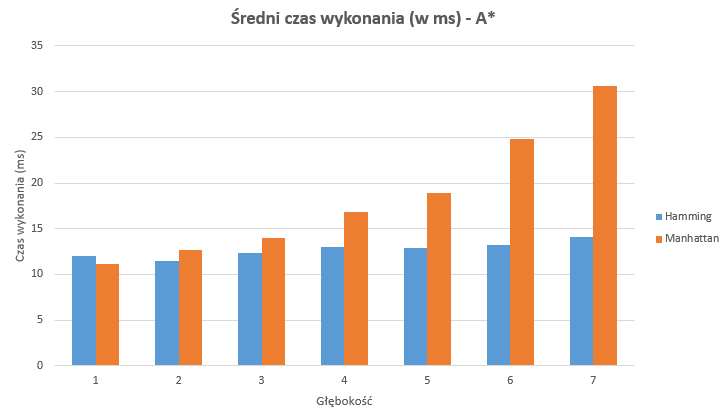
\includegraphics[width=0.85\textwidth]{czasastr.png}
    \caption{Średni czas wykonania dla algorytmu A*}
	\label{czasastr}
\end{figure}
\begin{figure}[h!]
    \centering
    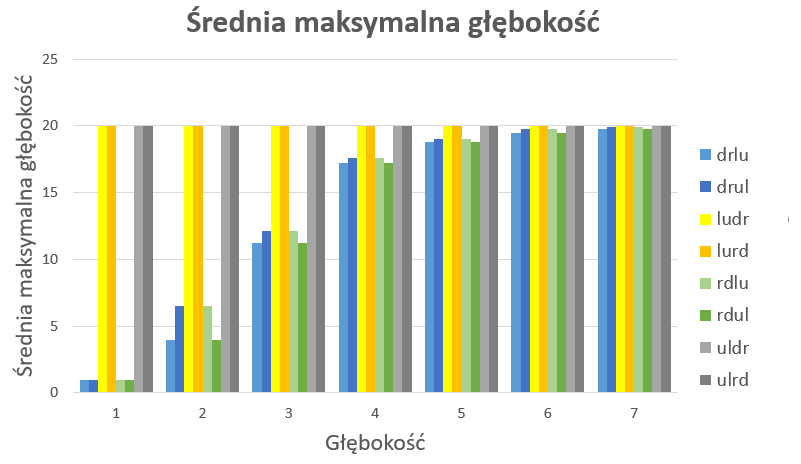
\includegraphics[width=0.83\textwidth]{maxdepthDFS.png}
    \caption{Średnia maksymalna głębokość dla algorytmu DFS}
	\label{maxdepthDFS}
\end{figure}
\begin{figure}[h!]
    \centering
    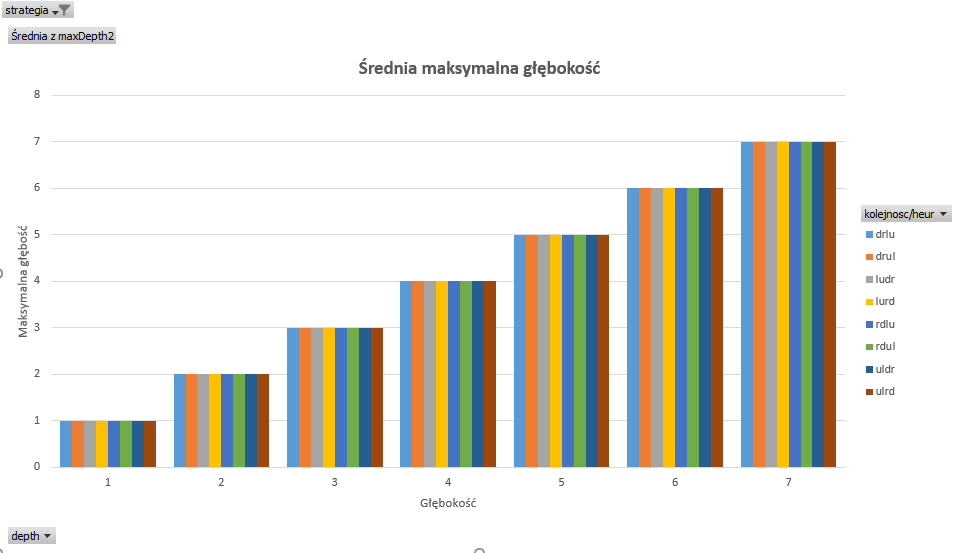
\includegraphics[width=0.83\textwidth]{maxdepthBFS.png}
    \caption{Średnia maksymalna głębokość dla algorytmu BFS}
	\label{maxdepthBFS}
\end{figure}
\begin{figure}[h!]
    \centering
    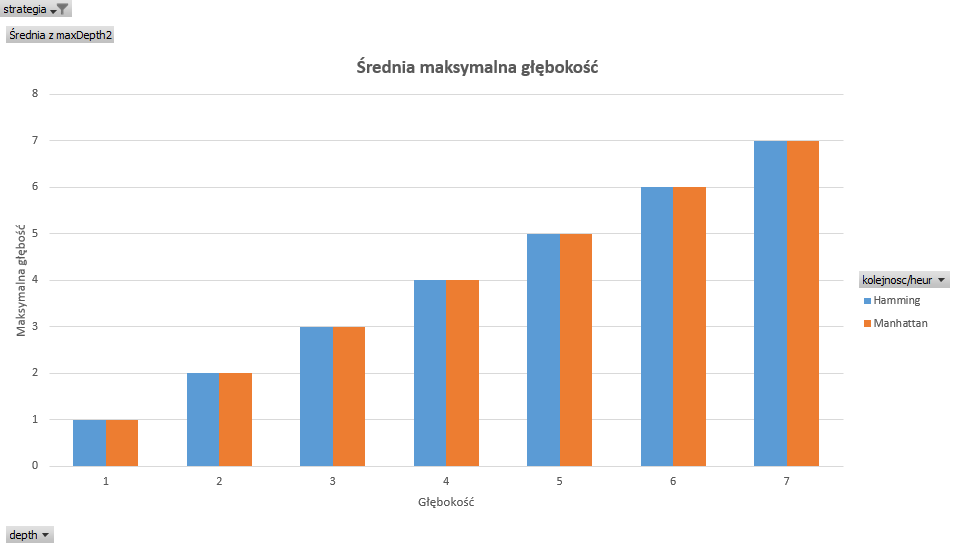
\includegraphics[width=0.83\textwidth]{maxdepthAstar.png}
    \caption{Średnia maksymalna głębokość dla algorytmu A*}
	\label{maxdepthAstar}
\end{figure}


\newpage
\section{Dyskusja}
{\color{blue}
Sekcja ta powinna zawierać dokładną interpretację uzyskanych wyników
eksperymentów wraz ze szczegółowymi wnioskami z nich płynącymi. Najcenniejsze
są, rzecz jasna, wnioski o charakterze uniwersalnym, które mogą być istotne
przy innych, podobnych zadaniach. Należy również omówić i wyjaśnić wszystkie
napotkane problemy (jeśli takie były). Każdy wniosek powinien mieć poparcie we
wcześniej przeprowadzonych eksperymentach (odwołania do konkretnych wyników).
Jest to jedna z najważniejszych sekcji tego sprawozdania, gdyż prezentuje
poziom zrozumienia badanego problemu.}

\section{Wnioski}
{\color{blue}
W tej, przedostatniej, sekcji należy zamieścić podsumowanie najważniejszych
wniosków z sekcji poprzedniej. Najlepiej jest je po prostu wypunktować. Znów,
tak jak poprzednio, najistotniejsze są wnioski o charakterze uniwersalnym.}

\begin{thebibliography}{0}
  	
	\bibitem{pierwszymath} \textsl{http://www.math.ubc.ca/~cass/courses/m308-02b/projects/grant/fifteen.html} [dostęp 17.03.2020]
	\bibitem{wikiDFS} \textsl{https://pl.wikipedia.org/wiki/Przeszukiwanie\_w\_głąb} [dostęp 17.03.2020]
	\bibitem{wikiBFS} \textsl{https://pl.wikipedia.org/wiki/Przeszukiwanie\_wszerz} [dostęp 17.03.2020]
	\bibitem{astr}		\textsl{https://en.wikipedia.org/wiki/A*\_search\_algorithm} [dostęp 17.03.2020]
\end{thebibliography}


\end{document}
